%\documentclass[12pt,manuscript]{aastex}
\documentclass[]{emulateapj}
\bibliographystyle{apj}
\usepackage{graphicx}
\usepackage[suffix=]{epstopdf}
\usepackage{natbib}
\usepackage{amsmath}
%         Make Scientific Notation
\providecommand{\e}[1]{\ensuremath{\times 10^{#1}}}
\usepackage{url} 

\shortauthors{Davenport et al.}
\shorttitle{2MASS Variability}

\begin{document}
 
\title{Stellar Variability from the 2MASS Calibration Scans}

\author{James R. A. Davenport\altaffilmark{1,2},
Andrew C. Becker\altaffilmark{2},
Peter Plavchan\altaffilmark{3},
Roc Cutri\altaffilmark{3}}

 
\altaffiltext{1}{Corresponding author: jrad@astro.washington.edu}
\altaffiltext{2}{Department of Astronomy, University of Washington, Box 351580, Seattle, WA 98195}
\altaffiltext{3}{Infrared Processing and Analysis Center, California Institute of Technology, Pasadena, CA 91125, USA}



\begin{abstract}
data comes from 2mass-calpswdb, have over 100 million photometric measurements, totaling light curves for 113,030 point objects. we have run supersmoother period folding, ala MACHO, on every light curve. By hand verification used to check. many are found periodic, XX binaries, YY radial pulsators. These include the best sampled light curves for an RR Lyr and Cepheid variables in the NIR, and provide an important benchmark for modeling of these stars. An additional ZZ quasi-periodic variable stars are found. we have also characterized the variability properties as functions of color, finding nearly all objects have ``grey'' variability, where the amplitude is independent of wavelength chosen.
\end{abstract}


\keywords{variability, surveys, NIR}


%%%%%%%%%%%%%%%%%%%%%%%%%
\section{Introduction}
Arguably the two greatest advancements in optical and infrared photometric surveys within the past two decades have been 1) the advent of 1\% accurate multi-wavelength photometry for contiguous portions of the sky exceeding $\Omega\sim10^5$ deg$^2$, and 2) time resolved surveys spanning days to years baselines. As both the temporal and spatial domains are explored, new astrophysical phenomena are uncovered, while the previously rare events are placed in a statistical context. Naturally, the next generation survey will exploit both of these domains simultaneously, producing deep multi-wavelength surveys with both unprecedented spatial and temporal coverage. In order to prepare for these future surveys, which will contain orders of magnitude larger numbers of  variable sources, we must hone our skills using existing catalogs/databases. This will precipitate the development of new techniques, and inform the targeting, cadence, and observing strategies of the many future time domain surveys.

WISE will provide huge variability data in the mid IR for regions near the orbital poles. Many papers using NIR variability to study new physics. The VVV (VISTA variables in the V{\'{\i}}a L{\'a}ctea) survey in the bulge, DR1 just release \citep{vvv_dr1}

The Two Micron All Sky Survey \citep[2MASS;][]{2mass} imaged the full sky in three, simultaneously obtained, near-infrared (NIR) bands. Survey operations were conducted between 1997 and 2001, using a northern and southern telescope. Photometric calibration for 2MASS was accomplished using repeated observations of 35 selected fields, which were spaced across the sky \citep{nikolaev2000}. An additional 5 tiles were imaged around the Large and Small Magellanic Clouds during the last year of operation. Each calibration field covered an area of approximately 8\farcm5 (RA) $\times 1^\circ$ (Dec). The 35 standard calibration fields were scanned ranging between 562 and 3,692 times over the 4 year period, yielding some of the best NIR light curves yet produced. The placement of these tiles is shown in Figure \ref{radec}, and they contain light curves for approximately 110,000 point source objects.


These calibration data have been used for only a handful of studies to date. 
\citet{plavchan2008a} characterized many of the details in analyzing this unique dataset for time domain studies. They also mined these data for periodic objects, finding 3 new M dwarf eclipsing binaries. 
\citet{plavchan2008b} studied the 131 day periodic object, 2MASS J16271848--2429059, revealing a possible three-body YSO system. 
\citet{sarajedini2009} utilized the images from multiple scans of calibration tile 90067 to produce a NIR color-magnitude diagram for the open cluster M67 that probed $\gtrsim$3 magnitudes deeper than the standard 2MASS point source catalog. 
\citet{becker2008} discovered and characterized a 2.6 d M dwarf binary, 2MASS J01542930+0053266. This system was located in both the 2MASS calibration tile 90004, and the ``Stripe 82'' region of the Sloan Digital Sky Survey \citep[SDSS;][]{york2000} footprint, which yielded an 8-band light curve ($ugrizJHK_s$) for the binary. 
Using 16 of the calibration tiles that overlapped the SDSS footprint, \citet{davenport2012} produced some of the first constraints on the properties of M dwarf flares in red optical and NIR bandpasses. 


MENTION THESE TWO? 
(P. Plavchan 2012 submitted) an analysis of a 92 day periodic YSO. 
(J. Parks 2012 submitted) a detailed study of the $\rho$ Ophiuchus star forming region tile. 


In this paper we present a census of the variable stellar objects from this 4 year NIR survey. The data and period finding methodology is outlined in \S2. We describe the selection and classification of binary stars and radial pulsating objects in \S3. Quasi-periodic and other large amplitude variables that were recovered are discussed in \S4. We examine the general variability characteristics of point sources in the 2MASS calibration scans in \S5, and concluding remarks are given in \S6.



%%%%%%%%%%%%%%%%%%%%%%%%%
\vspace{.1in}

\section{Data}


\begin{figure*}[!t]
\centering
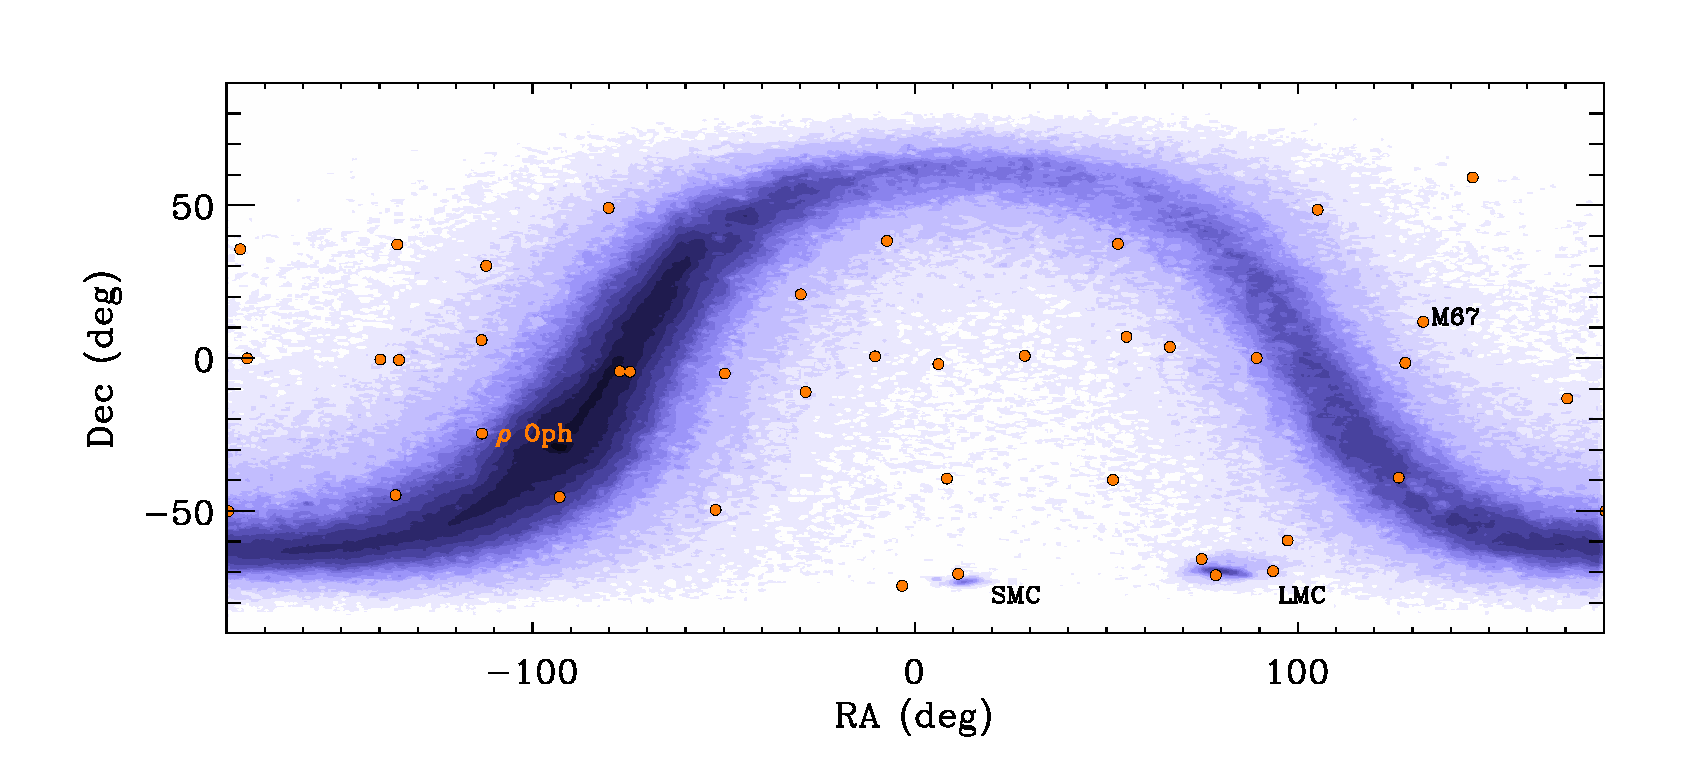
\includegraphics[width=7.0in]{new_plots/radec_psc}
\caption{Spatial distribution of the 40 Cal-PSWDB tiles (orange circles), with titles for a few notable tiles labeled. Background contours denote increasing density from a sample of 3 million randomly drawn point sources from the 2MASS point source catalog, and trace the Galactic plane, bulge, and the Large and Small Magellanic Clouds.}
\label{radec}
\end{figure*}

\vspace{.01in}



\begin{figure*}[!t]
\centering
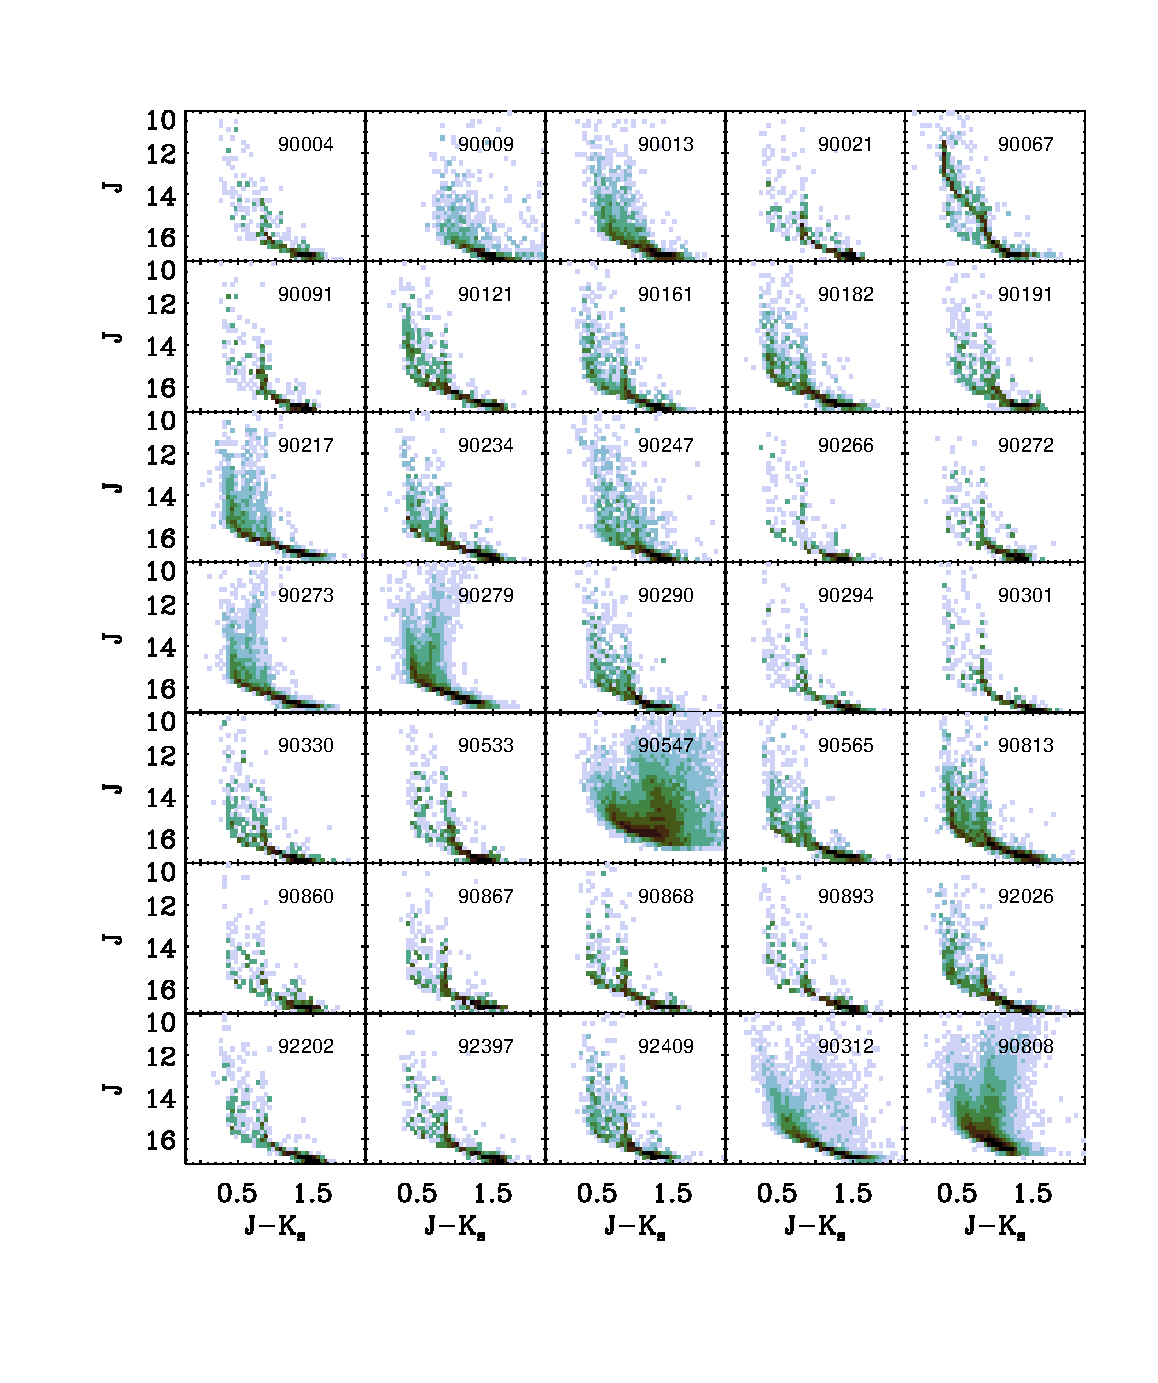
\includegraphics[width=7.0in]{new_plots/big_cmd1}
\caption{color mag diagrams for the fields}
\label{cmd1}
\end{figure*}
\clearpage

\begin{figure*}[!t]
\centering
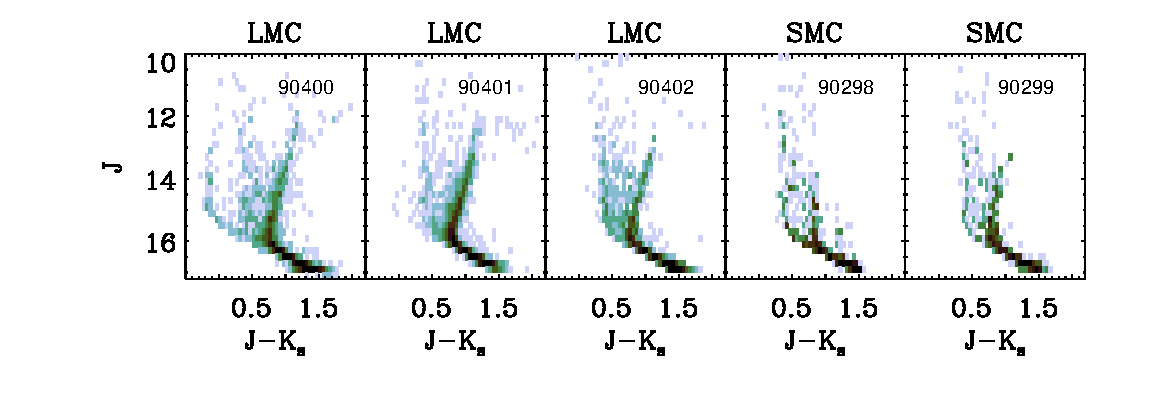
\includegraphics[width=7.0in]{new_plots/big_cmd2}
\caption{color mag diagrams for the LMC/SMC fields}
\label{cmd2}
\end{figure*}


lots of testing, characterization of the Cal-PSWDB done in \citep{plavchanphd,plavchan2008a}
Each night during 2MASS operations, the survey telescopes were directed at one of the calibration fields once per hour (before 1997 October 11 UT two fields were observed every 2 hours). During each visit, six consecutive scans of the field were made in alternating declination directions in $\sim$10 minutes of elapsed real time (a ��scan group��). Each scan in the set of six was offset from the preceding scan by $\sim$5" in R.A. to avoid systematic pixel effects. The calibration fields were observed using the same ��freeze-frame�� scanning strategy used for the main survey that yielded a net 7.8 s exposure on the sky per scan. Over the course of the 2MASS survey, between 562 and 3692 independent observations were made of each of the 35 calibration fields. Table 1 presents a list of these fields and their aggregate properties.



The raw imaging data from each scan of a 2MASS calibration field were reduced using the same automated data processing system used to process the survey observation data \citep{cutri2006}
(Cutri et al. 2006, Section IV ). The reduction process detected and extracted source positions and photometry for all objects in the images from each scan. Measurements of the standard stars in each field were used to determine the nightly photometric zero-point solutions as a function of time, and seasonal atmospheric coefficients. All source extractions from all scans were loaded into the 2MASS Calibration Point Source Working Database (Cal-PSWDB). This database contains over 191 million source extractions derived from 73,230 scans of the 35 calibration fields. Further descriptions of the Cal- PSWDB and its properties can be found in Cutri et al. (2006).


we ran the data through optics, got XX objects.

each light curve was processed with supersmsoother

objects with periods in at least 2 bands that were not obviously aliases were grabbed (about 2000 objects)

each light curve was examined by eye, about 250 were bona fide good periodic objects





%%%%%%%%%%%%%%%%%%%%%%%%%
\section{Periodic Variables}
searched all 2000 light curves of periodic things by eye to pick out the real ones. found correct periods by hand

this is a good data set to be used for training automated light curve morphology identification routines, provides benchmark objects of many types in the NIR


%identify object type using fourier modes

Eclipsing binaries and pulsating variables can be separated and classified by fitting fourier modes to the light curves \citep{pojmanski2002,nefs2012}.

To separate binaries from pulsators, we cut on:
\begin{equation}
b_1({\rm binary}) \ge  -0.13\left( \frac{a_4}{a_2} \right)- 0.3
\end{equation}

and different configurations of binaries can be determined using:
\begin{eqnarray}
a_4({\rm detached}) \ge & a_2(0.5 + a_2)\\
a_4({\rm contact}) \le & a_2(0.125 + a_2)
\end{eqnarray}




\begin{figure}[]
\centering
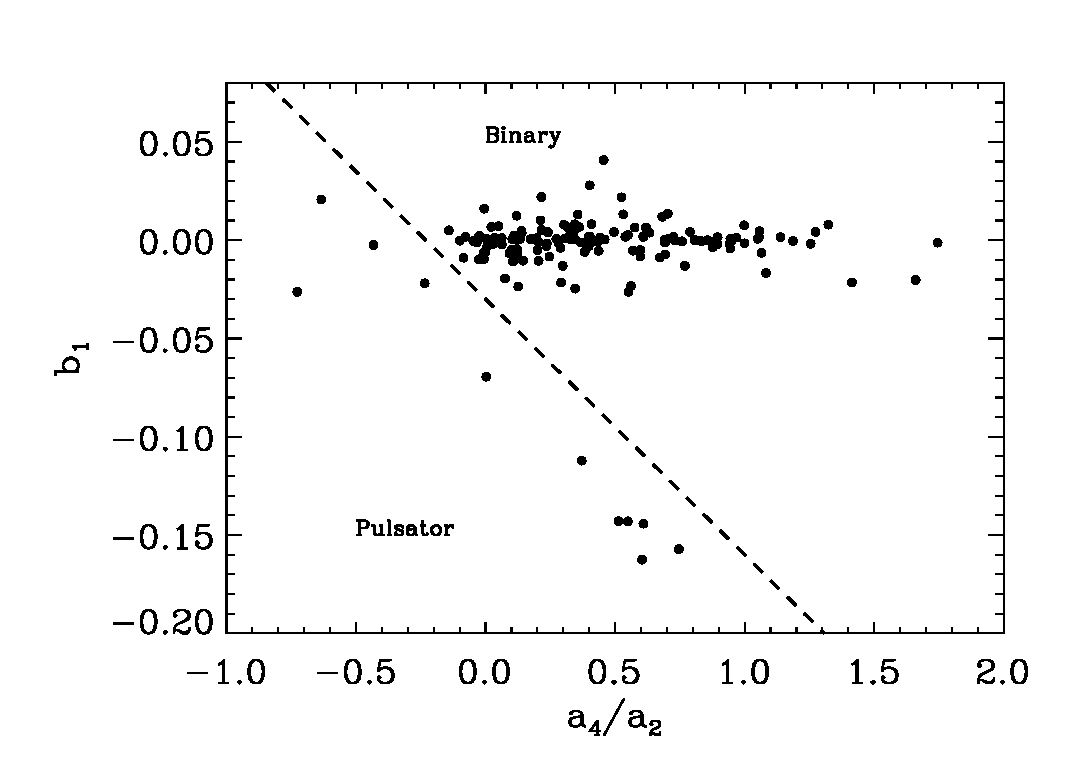
\includegraphics[width=3.5in]{new_plots/four_a42b1}
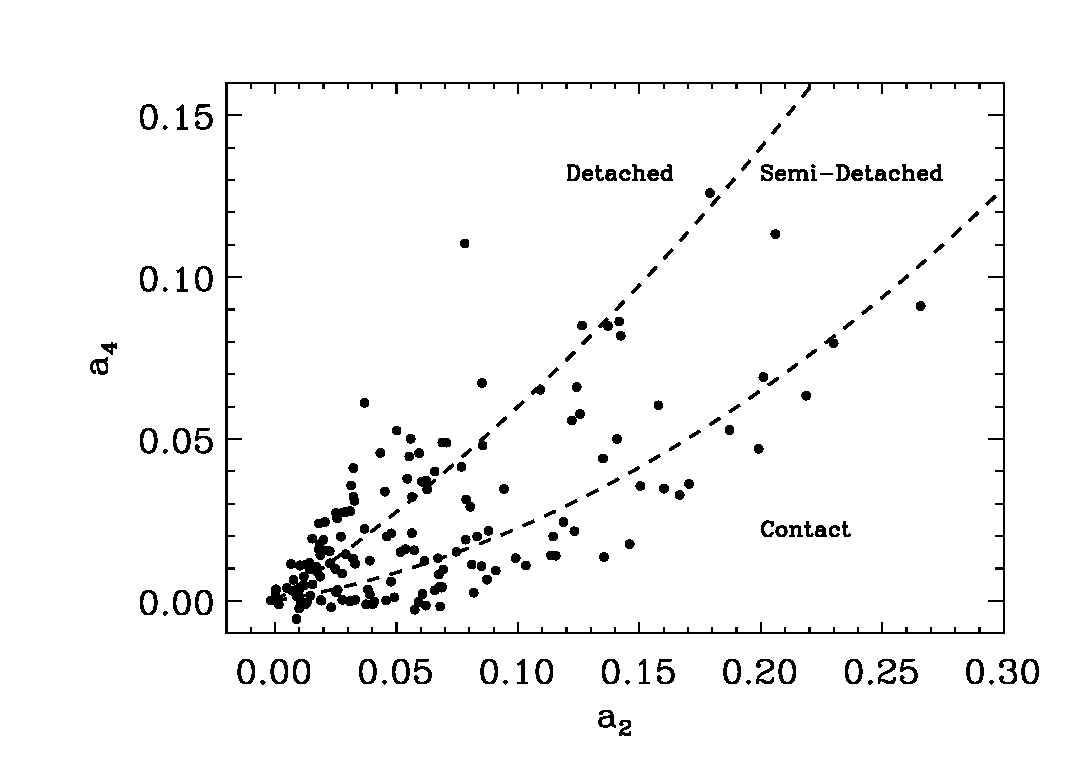
\includegraphics[width=3.5in]{new_plots/four_a2a4}
\caption{Fourier modes used to select between eclipsing binaries and pulsators (top) and different classes of eclipsing binaries (bottom).}
\label{four_bb}
\end{figure}


%%%%%%%%%%%%%%%%%%%%%%%%%
\subsection{Binaries}
We found 100 binaries, need a histogram of their periods. We recover nearly all the binaries from Plavchan's early work (8/23 missed so far)

\input{bb_table}


match to new paper by J Parks (2012)

for every binary, estimate the spectral type based on my color-locus

\begin{figure}[]
\centering
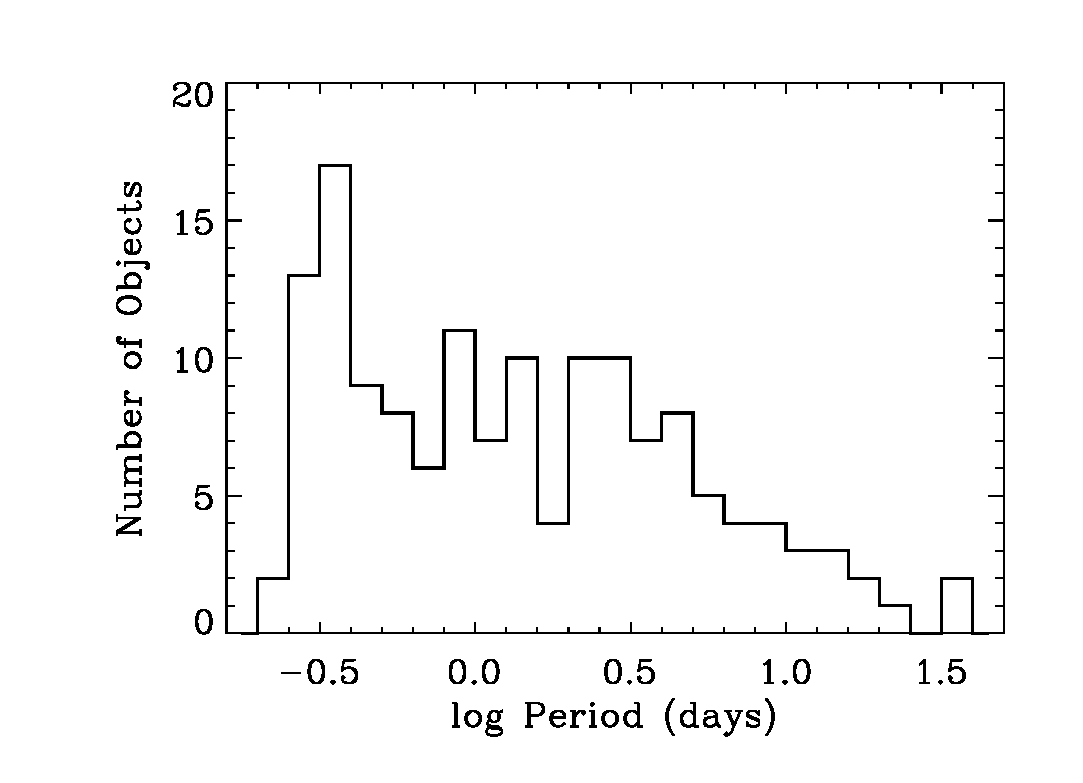
\includegraphics[width=3.5in]{new_plots/bb_perhist}
\caption{Histogram of objects selected as binaries.}
\label{perhist}
\end{figure}



\begin{figure}[!h]
\centering
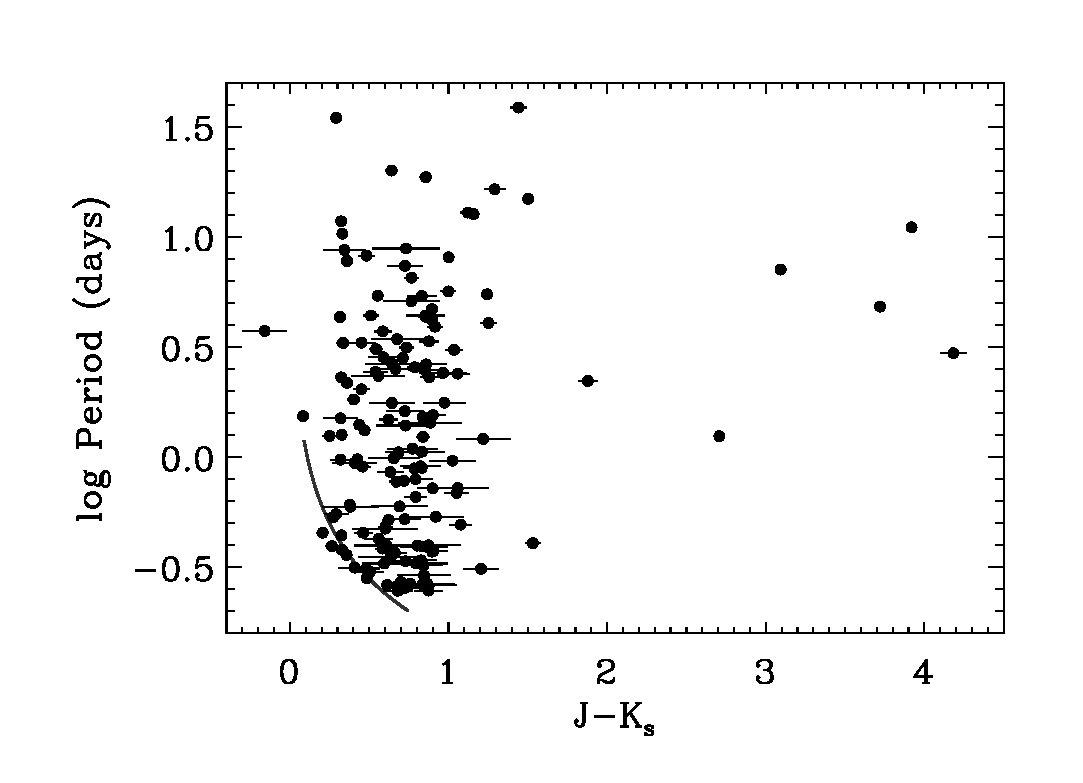
\includegraphics[width=3.5in]{new_plots/color_period_bb}
\caption{Period versus median colors for objects selected as binaries. The photometry was not corrected for reddening. The power law short period contact binary limit from \cite{deb2011} is shown for comparison (solid grey line).}
\label{periods}
\end{figure}



\begin{figure*}[]
\centering
\includegraphics[width=2.0in]{plots/bb1_3}
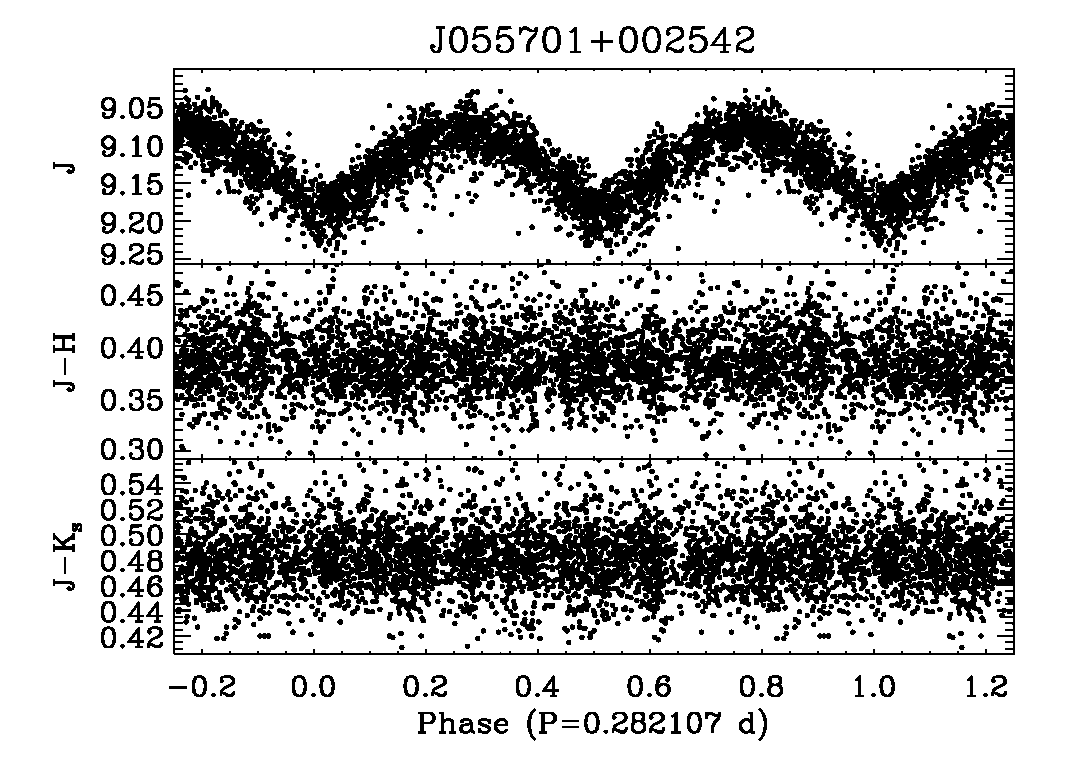
\includegraphics[width=2.0in]{plots/bb1_4}
\includegraphics[width=2.0in]{plots/bb1_5}\\
\includegraphics[width=2.0in]{plots/bb1_6}
\includegraphics[width=2.0in]{plots/bb1_44}
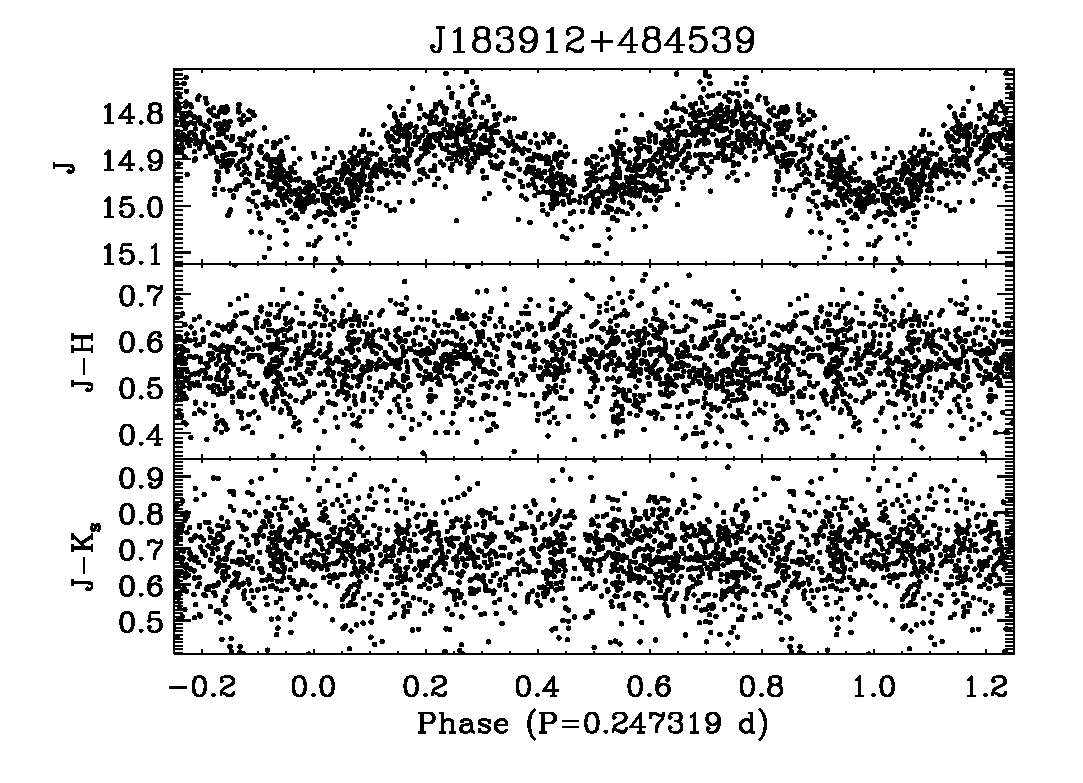
\includegraphics[width=2.0in]{plots/bb1_13}\\
\includegraphics[width=2.0in]{plots/bb1_14}
\includegraphics[width=2.0in]{plots/bb1_22}
\includegraphics[width=2.0in]{plots/bb1_27}
\caption{detached binaries}
\label{bin1}
\end{figure*}


\begin{figure*}[]
\centering
\includegraphics[width=2.0in]{plots/bb2_1}
\includegraphics[width=2.0in]{plots/bb2_2}
\includegraphics[width=2.0in]{plots/bb2_7}\\
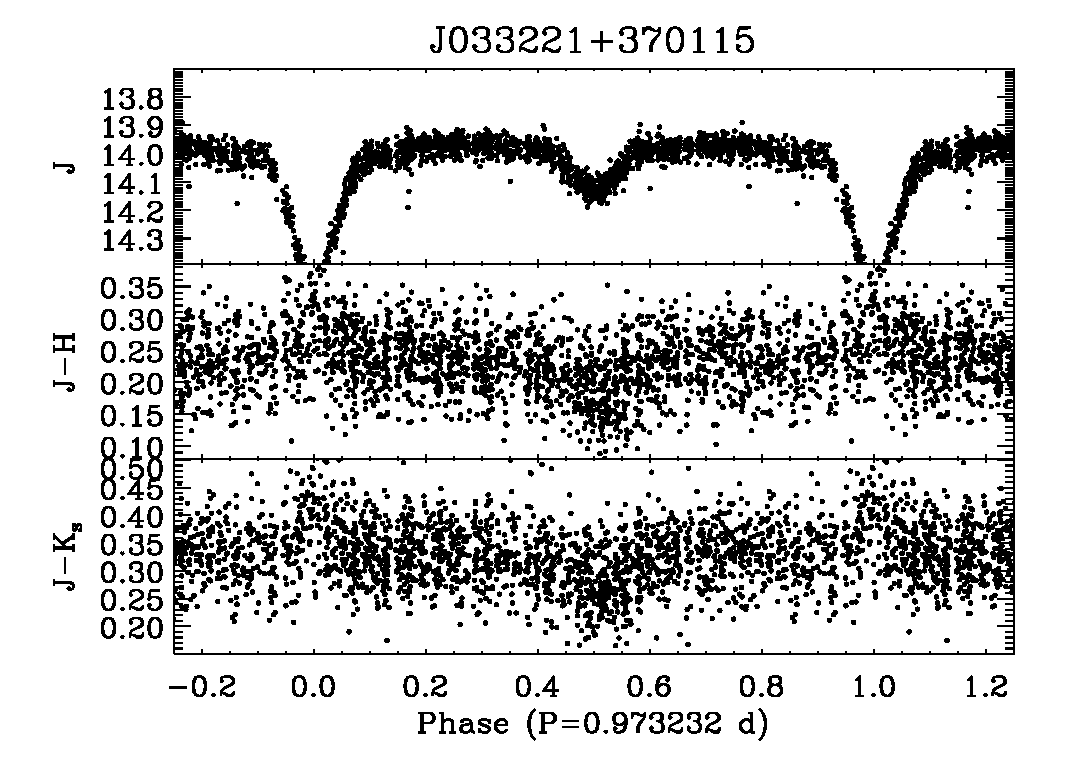
\includegraphics[width=2.0in]{plots/bb2_8}
\includegraphics[width=2.0in]{plots/bb2_11}
\includegraphics[width=2.0in]{plots/bb2_13}\\
\includegraphics[width=2.0in]{plots/bb2_19}
\includegraphics[width=2.0in]{plots/bb2_28}
\includegraphics[width=2.0in]{plots/bb2_30}\\
\includegraphics[width=2.0in]{plots/bb2_31}
\includegraphics[width=2.0in]{plots/bb2_45}
\includegraphics[width=2.0in]{plots/bb2_46}
\caption{detached binaries}
\label{bin1}
\end{figure*}


\begin{figure}[]
\centering
\includegraphics[width=3.0in]{plots/shortest_sep}
\caption{detached binaries}
\label{shortbin}
\end{figure}




%%%%%%%%%%%%%%%%%%%%%%%%%
\subsection{Pulsators}
Infrared observations of radial pulsating stars was first performed by \cite{wisniewski1968}, and detailed characterization was done for Cepheid variables by \cite{mcgonegal1982} and for RR Lyr variables by \cite{longmore1985}

$K$-band templates first derived in \citet{jones1996}

\citet{sollima2008} produced $JHK_s$ light curves for the prototypical star, RR Lyr.

\begin{deluxetable*}{lccccccccccc}
%\rotate
\setlength{\tabcolsep}{0.02in} 
\tabletypesize{\tiny}
\tablecolumns{12}
\tablecaption{The catalog of radial pulsating type periodic variables, selected using Fourier modes.}
\tablehead{
	\colhead{ObjectID}&
	\colhead{FieldID} &
	\colhead{RA} &
	\colhead{Dec} &
	\colhead{Period} &
	\colhead{$\langle J\rangle$} &
	\colhead{$\langle H\rangle$} & 
	\colhead{$\langle K_s\rangle$} &
	\colhead{\# epochs} &
	\colhead{$a_2$} &
	\colhead{$a_4$} &
	\colhead{$b_1$} \\
	\colhead{(hhmmss+ddmmss)}&
	\colhead{} &
	\colhead{(deg)} &
	\colhead{(deg)} &
	\colhead{(days)} &
	\colhead{(mag)} &
	\colhead{(mag)} & 
	\colhead{(mag)} &
	\colhead{} &
	\colhead{} &
	\colhead{} &
	\colhead{}
	}
\startdata
  J120137-494808 &  90217 &   180.40575 &   -49.80240 &    0.08777 & 15.22 & 15.03 & 14.95 &   1685 &  0.03441 & -0.14304 &  0.06262 \\
  J183913+492837 &  90182 &   279.80688 &    49.47710 &    0.37473 & 15.96 & 15.68 & 15.43 &   1682 &  0.01161 & -0.14297 &  0.02263 \\
  J174818-452629 &  90279 &   267.07571 &   -45.44157 &    0.41014 & 14.93 & 14.68 & 14.60 &    977 &  0.00012 & -0.00248 & -0.00028 \\
  J162725-250621 &  90009 &   246.85564 &   -25.10589 &    0.48514 & 15.46 & 14.98 & 14.82 &   1579 & -0.00560 &  0.02069 &  0.00883 \\
  J220009+211502 &  92409 &   330.04028 &    21.25065 &    0.51424 & 14.60 & 14.35 & 14.29 &     41 & -0.00234 & -0.02196 &  0.00994 \\
  J190144-042605 &  90808 &   285.43744 &    -4.43475 &    0.52396 & 15.61 & 15.14 & 14.97 &   1879 & -0.00112 & -0.02633 &  0.00154 \\
  J174835-452347 &  90279 &   267.14786 &   -45.39640 &    0.54504 & 15.63 & 15.35 & 15.22 &    972 &  0.02224 & -0.16258 &  0.03681 \\
  J015450+001501 &  90004 &    28.70900 &     0.25038 &    0.63698 & 14.27 & 14.01 & 13.98 &   2972 &  0.02093 & -0.11219 &  0.05638 \\
  J085107+115302 &  90067 &   132.78021 &    11.88394 &    0.67940 & 11.19 & 10.80 & 10.69 &   3692 &  0.03375 & -0.15717 &  0.04523 \\
  J082535-392008 &  90312 &   126.39848 &   -39.33574 &    3.07471 & 12.57 & 11.66 & 11.28 &   3501 &  0.00012 & -0.06949 &  0.04578 \\
  J174811-455323 &  90279 &   267.04904 &   -45.88993 &    6.45956 & 14.02 & 13.40 & 13.27 &    968 &  0.03683 & -0.14425 &  0.06046 
\enddata
\label{rrtable}
\end{deluxetable*}


\begin{figure}[]
\centering
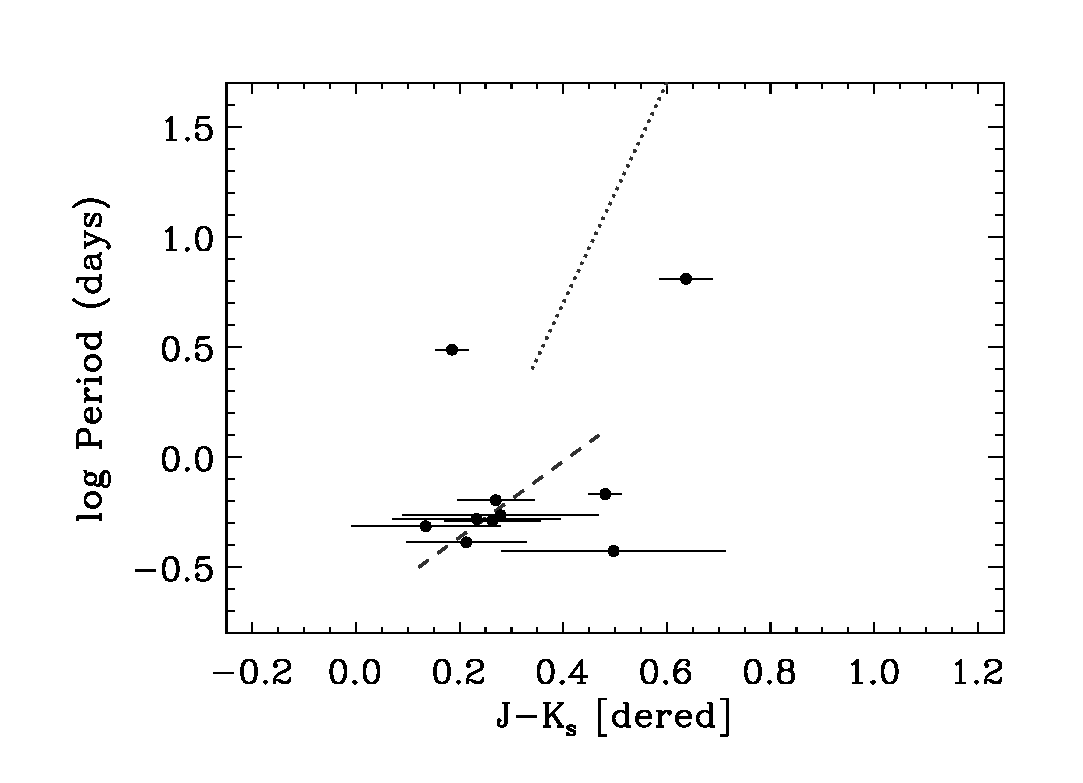
\includegraphics[width=3.0in]{new_plots/color_period_rr}
\caption{17 radial pulsator variables. dashed line is theoretical prediction from \citet{catelan2004} with Z=0.001 (no discernible dependence on Z) dotted line is for cepheids, from ...}
\label{rr_color_period}
\end{figure}



\begin{figure*}[]
\centering
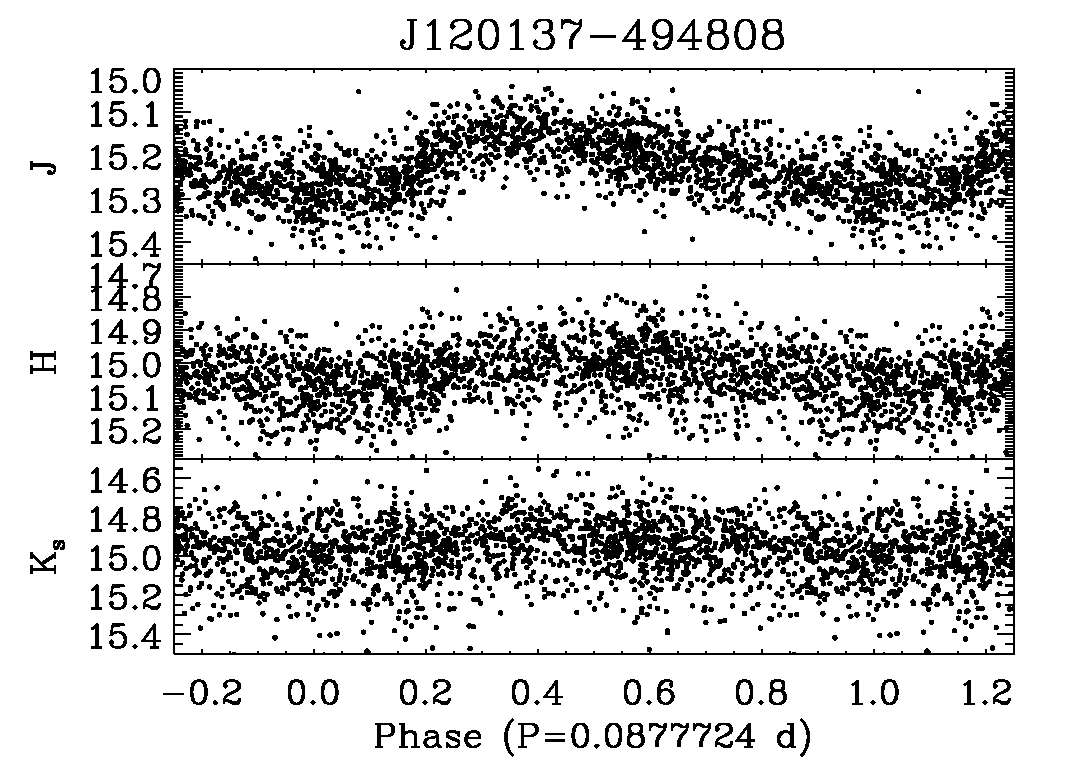
\includegraphics[width=2.0in]{new_plots/rr_0}
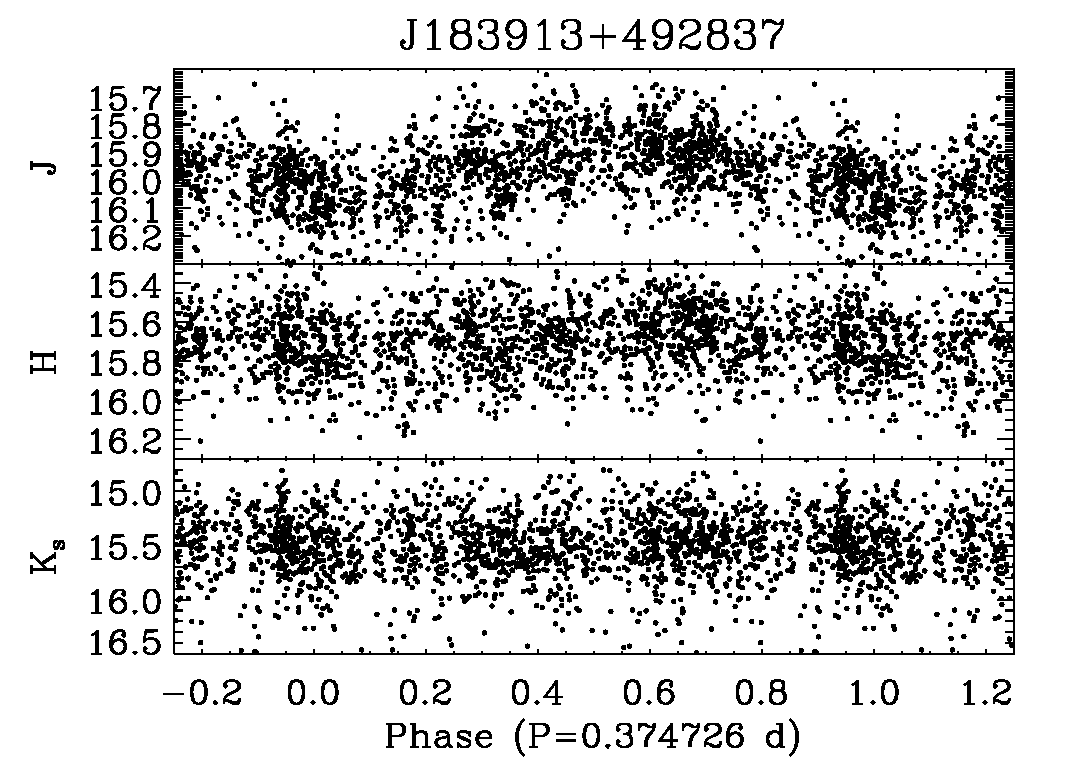
\includegraphics[width=2.0in]{new_plots/rr_1}
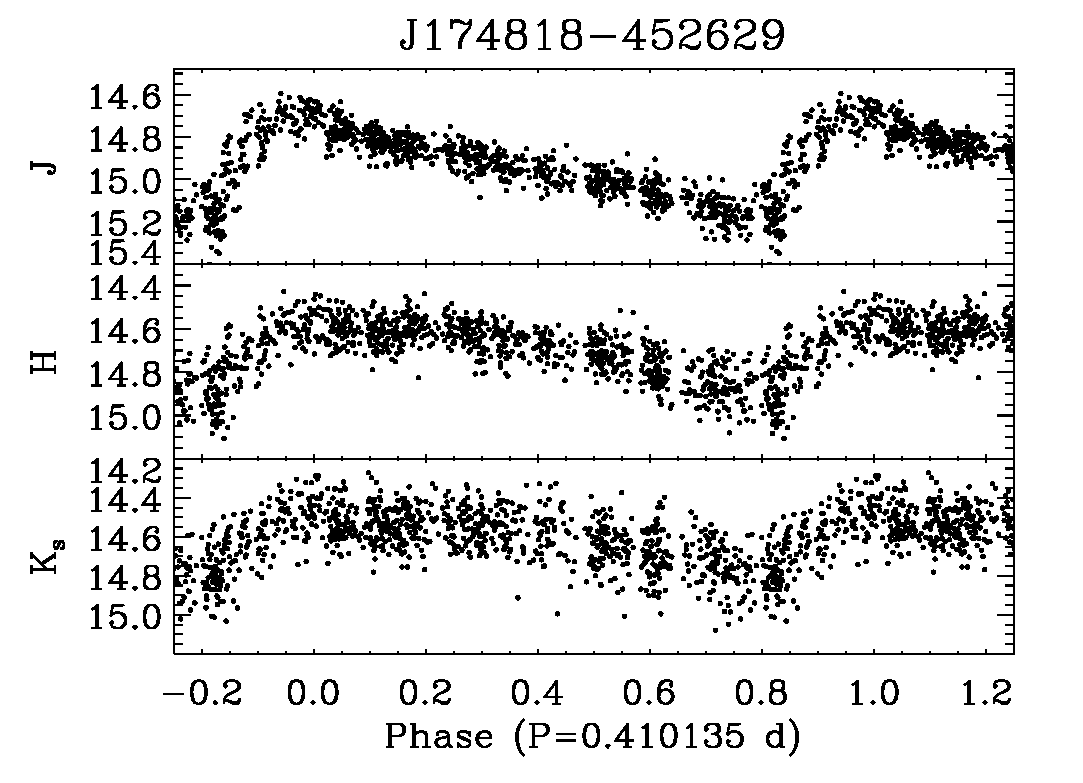
\includegraphics[width=2.0in]{new_plots/rr_2}\\
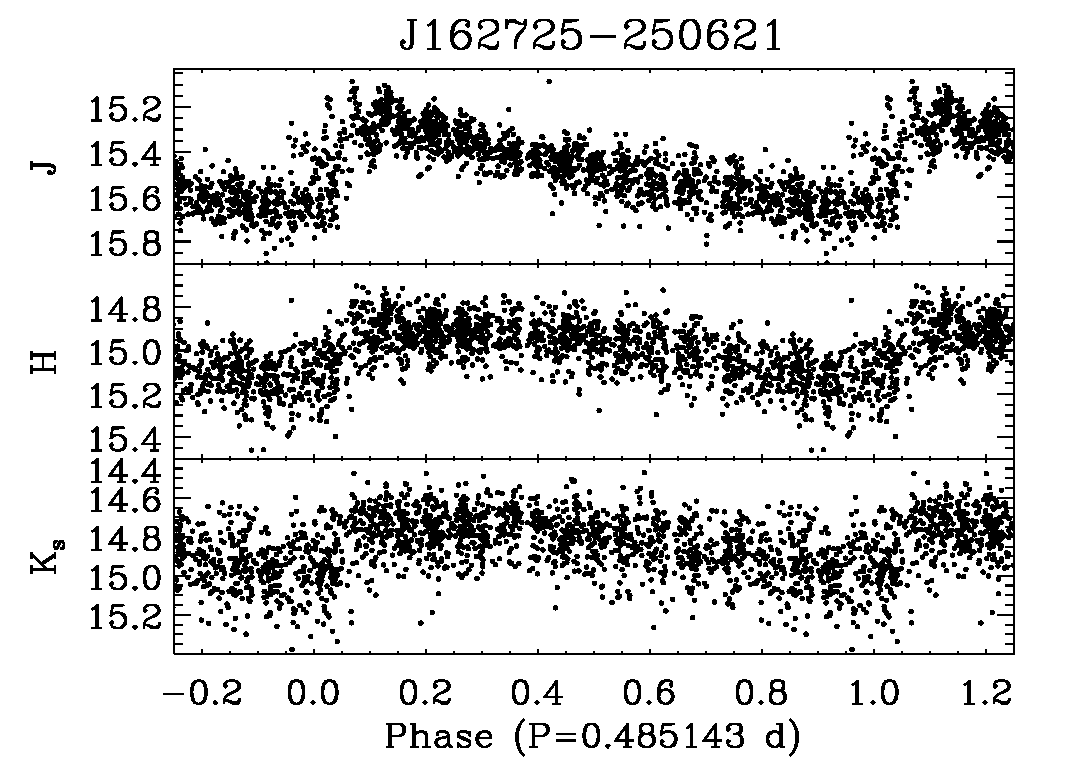
\includegraphics[width=2.0in]{new_plots/rr_3}
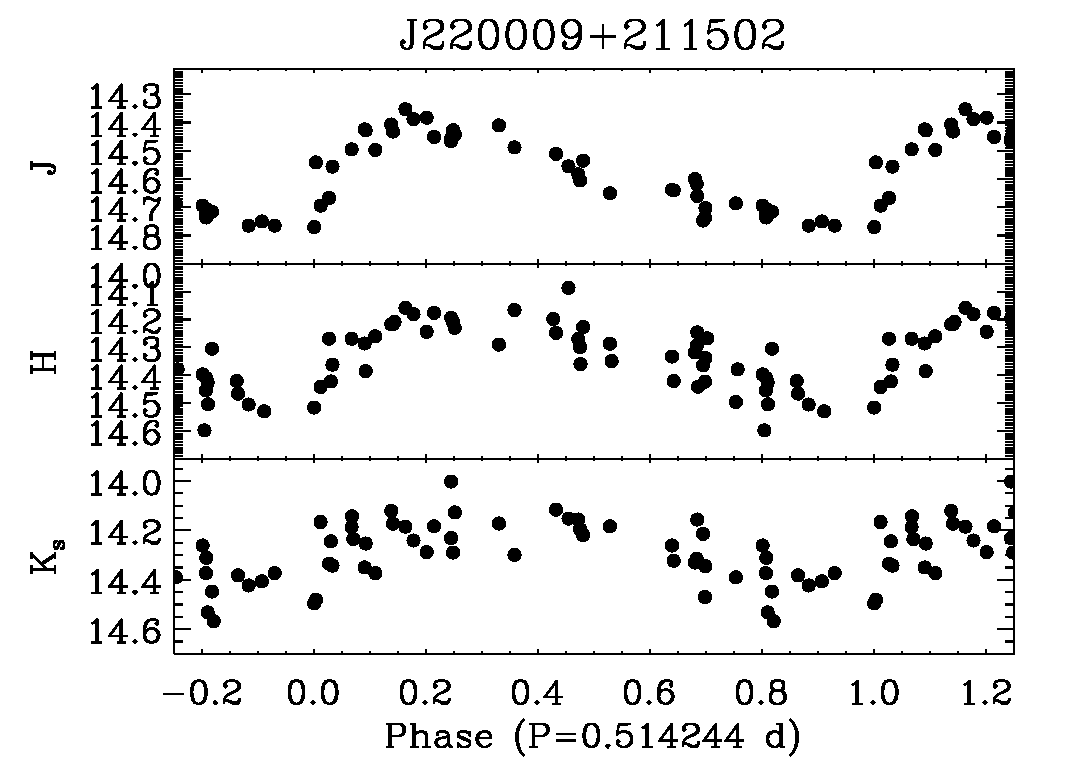
\includegraphics[width=2.0in]{new_plots/rr_4}
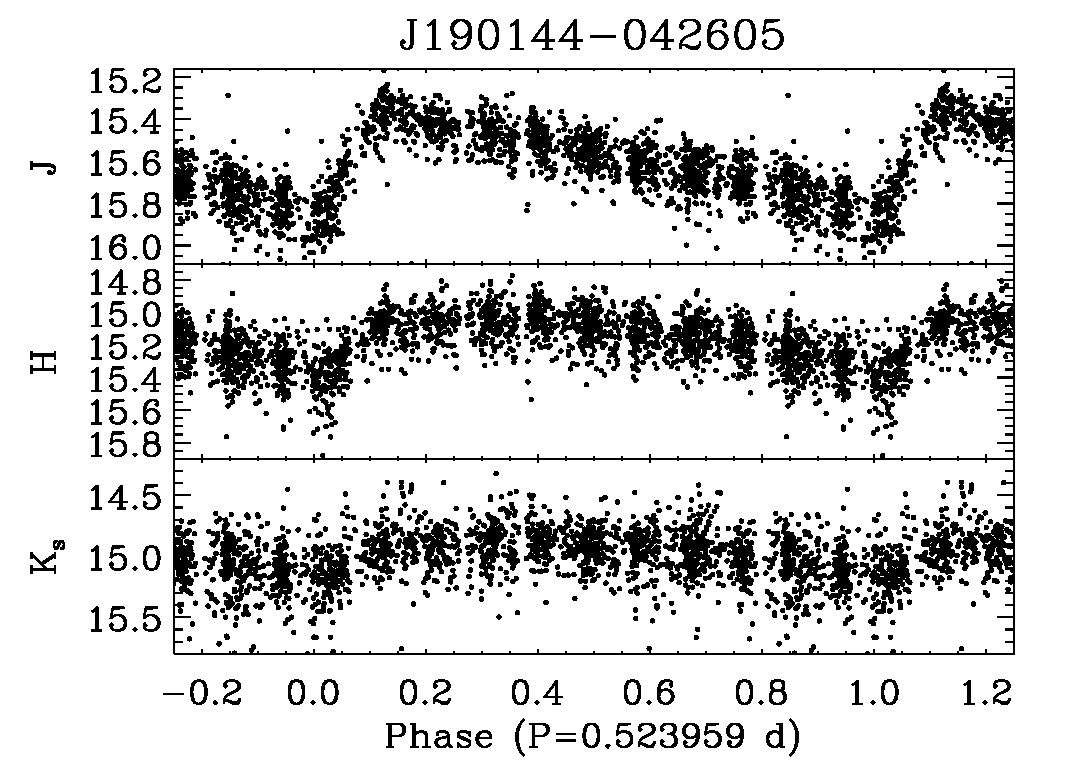
\includegraphics[width=2.0in]{new_plots/rr_5}\\
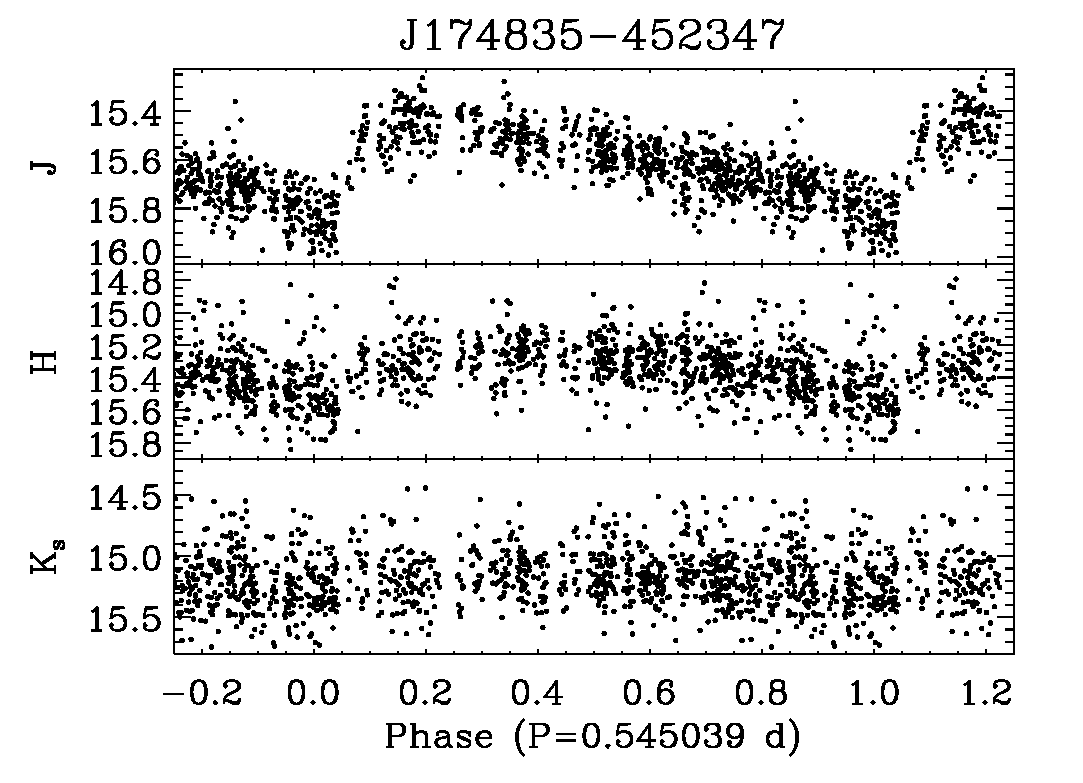
\includegraphics[width=2.0in]{new_plots/rr_6}
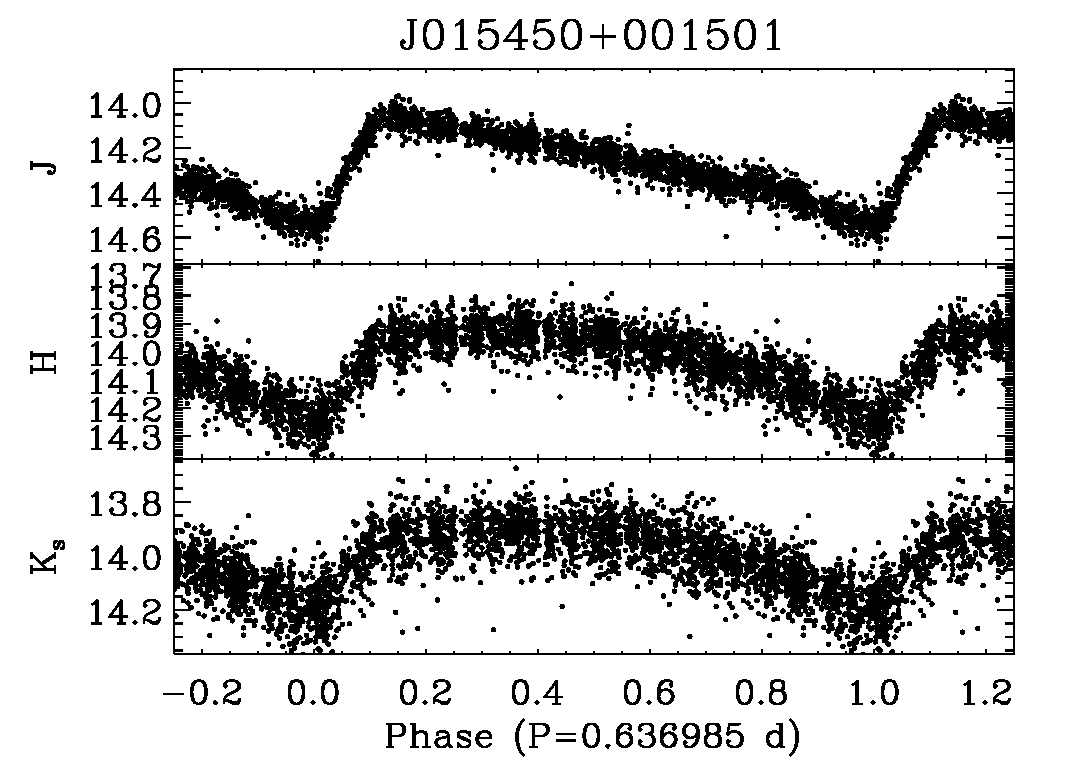
\includegraphics[width=2.0in]{new_plots/rr_7}
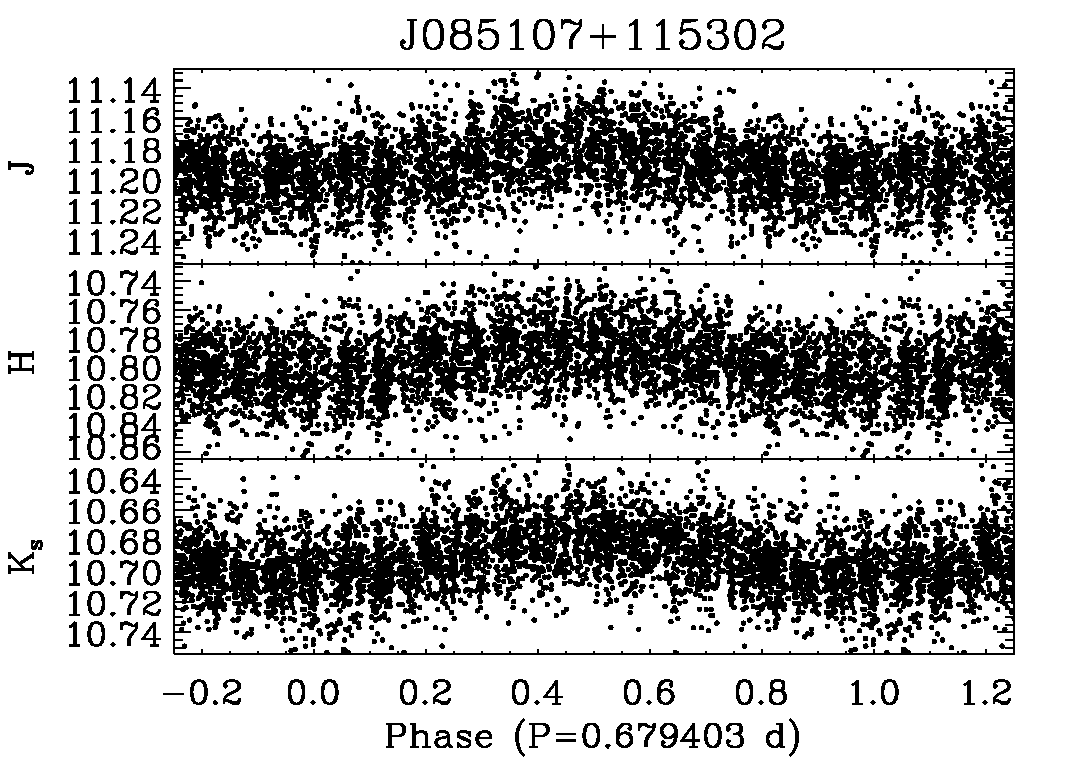
\includegraphics[width=2.0in]{new_plots/rr_8}
\caption{pulsators with periods less than 2 days (RR Lyr type)}
\label{rrshort}
\end{figure*}

\begin{figure*}[]
\centering
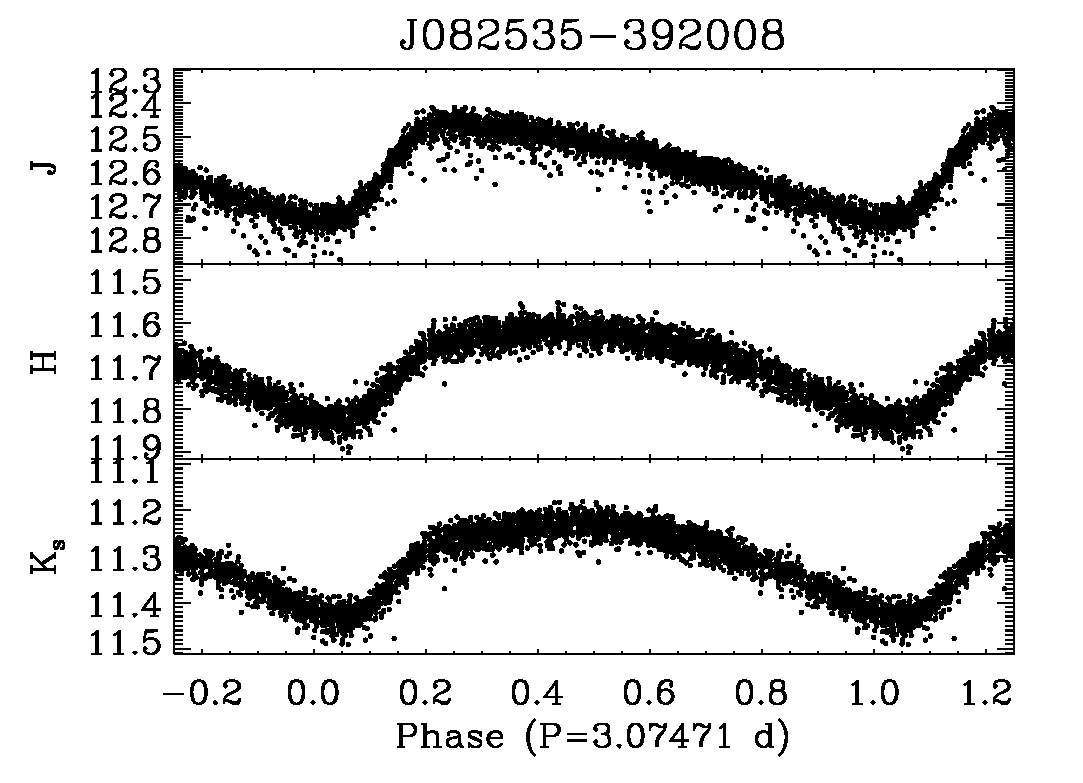
\includegraphics[width=2.5in]{new_plots/rr_9}
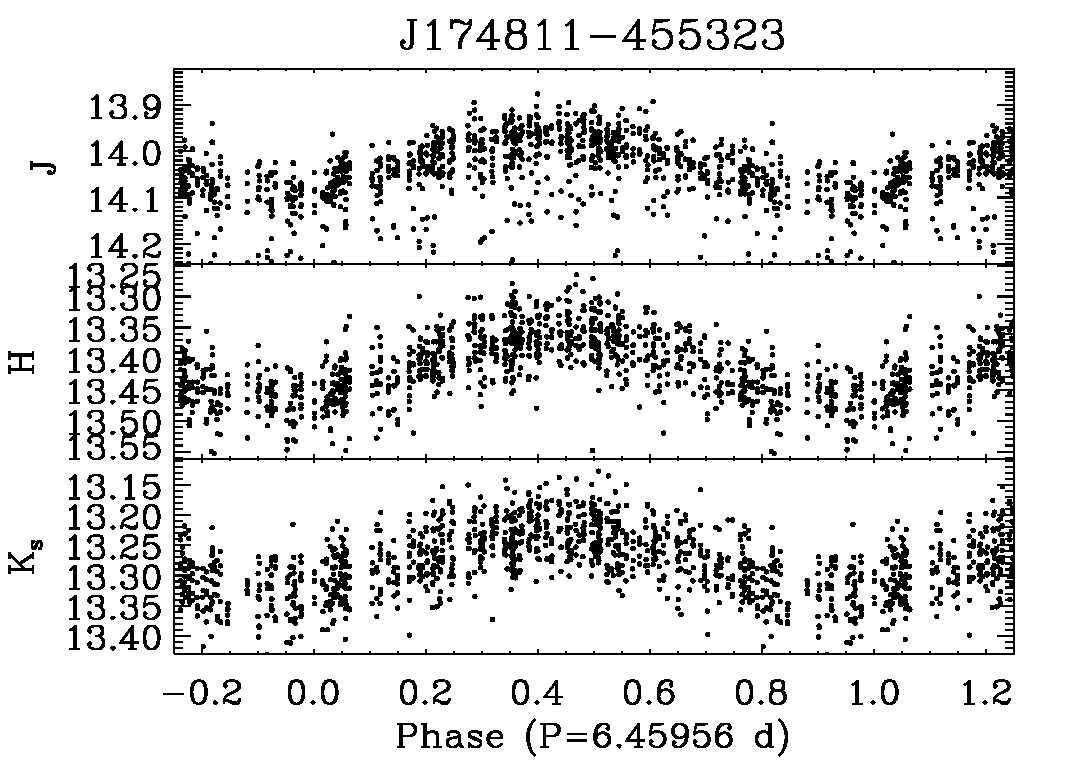
\includegraphics[width=2.5in]{new_plots/rr_10}
\caption{Pulsators (cepheids)  with periods longer than 2 days}
\label{rrlong}
\end{figure*}


\begin{figure*}[]
\centering
\includegraphics[width=3.0in]{plots/rr0_cmd}
\includegraphics[width=3.0in]{plots/rr15_cmd}
\caption{The color--magnitude evolution as a function of pulsation phase for the best sampled RR Lyr (top) and Cepheid (bottom) stars in our sample.}
\label{rrlyr2}
\end{figure*}



%%%%%%%%%%%%%%%%%%%%%%%%%
\section{Non-periodic Variables}
Plavchan and student have done lots of work on this for $\rho$ Oph field. We will only add other things that were identified by hand

\begin{deluxetable*}{lccccccccccc}
%\rotate
\setlength{\tabcolsep}{0.02in} 
\tabletypesize{\tiny}
\tablecolumns{11}
\tablecaption{The catalog of quasi-periodic variables. (THIS TEX FILE NEEDS TO BE REVISED TO ONLY INCLUDE THE ACTUALLY INTERESTING OBJECTS, MOST ARE ALREADY SHOWN)}
\tablehead{
	\colhead{ObjectID}&
	\colhead{FieldID} &
	\colhead{RA} &
	\colhead{Dec} &
	\colhead{$\langle J\rangle$} &
	\colhead{$\langle H\rangle$} & 
	\colhead{$\langle K_s\rangle$} &
	\colhead{\# epochs} &
	\colhead{$\sigma_J$} &
	\colhead{$\sigma_H$} &
	\colhead{$\sigma_K$} \\
	\colhead{(hhmmss+ddmmss)}&
	\colhead{} &
	\colhead{(deg)} &
	\colhead{(deg)} &
	\colhead{(mag)} &
	\colhead{(mag)} & 
	\colhead{(mag)} &
	\colhead{} &
	\colhead{(mag)} &
	\colhead{(mag)} &
	\colhead{(mag)}
	}
\startdata
  J162659-243556 &  90009 &   246.74608 &   -24.59911 & 16.40 & 13.45 & 11.86 &   1543 &  0.01401 &  0.00569 &  0.00182 \\
  J162722-244807 &  90009 &   246.84578 &   -24.80195 & 10.92 &  9.83 &  9.34 &   1581 & -0.00000 & -0.00000 &  0.00046 \\
  J162718-245453 &  90009 &   246.82655 &   -24.91494 & 11.42 & 10.54 &  9.95 &   1567 &  0.07128 &  0.04564 &  0.02912 %\\
%  J085113+115140 &  90067 &   132.80576 &    11.86123 & 11.59 & 11.04 & 10.91 &   3692 &  0.00051 &  0.00021 &  0.00008 \\
%  J070115+482309 &  90161 &   105.31503 &    48.38600 & 14.97 & 14.29 & 13.96 &   2576 &  0.00321 &  0.00378 &  0.00257 \\
%  J183935+485234 &  90182 &   279.89651 &    48.87616 & 12.54 & 11.94 & 11.80 &   1703 &  0.00011 &  0.00009 &  0.00001 \\
%  J120151-495519 &  90217 &   180.46277 &   -49.92199 & 15.08 & 14.43 & 14.28 &   1687 &  0.00265 &  0.00226 &  0.00266 \\
%  J145636-444345 &  90273 &   224.15221 &   -44.72928 & 16.45 & 15.87 & 15.41 &   1592 &  0.02448 &  0.00069 & -0.00000 \\
%  J145709-444631 &  90273 &   224.29086 &   -44.77550 &  8.07 &  7.12 &  6.74 &   1780 & -0.00000 & -0.00000 & -0.00000 \\
%  J174802-450540 &  90279 &   267.01227 &   -45.09446 &  9.61 &  8.66 &  8.30 &    961 &  0.00008 & -0.00000 &  0.00001 \\
%  J174805-452207 &  90279 &   267.02106 &   -45.36878 &  9.21 &  8.27 &  7.92 &    970 &  0.00048 & -0.00000 & -0.00000 \\
%  J174815-450235 &  90279 &   267.06516 &   -45.04307 & 10.70 &  9.76 &  9.43 &    975 &  0.00036 &  0.00015 &  0.00023 \\
%  J174827-451826 &  90279 &   267.11459 &   -45.30724 &  9.72 &  8.76 &  8.35 &    978 &  0.00030 & -0.00000 &  0.00043 \\
%  J174838-451704 &  90279 &   267.16211 &   -45.28449 & 10.28 &  9.38 &  9.13 &    977 &  0.00076 &  0.00066 &  0.00077 \\
%  J045901-655830 &  90400 &    74.75442 &   -65.97512 & 13.09 & 11.50 & 10.25 &    377 &  0.03248 &  0.02343 &  0.01467 \\
%  J045923-654151 &  90400 &    74.84740 &   -65.69778 & 11.68 & 11.70 & 11.70 &    378 &  0.00055 &  0.00057 &  0.00082 \\
%  J045929-651532 &  90400 &    74.87146 &   -65.25909 & 11.64 & 11.27 & 11.15 &    378 &  0.00132 &  0.00115 &  0.00081 \\
%  J051429-703352 &  90401 &    78.62468 &   -70.56453 & 13.97 & 13.58 & 13.49 &    156 &  0.00281 &  0.00201 &  0.00236 \\
%  J185106-044436 &  90547 &   282.77625 &    -4.74352 & 14.73 & 13.97 & 13.70 &    656 &  0.00448 &  0.00353 &  0.00138 \\
%  J185103-035333 &  90547 &   282.76584 &    -3.89267 & 14.37 & 13.28 & 12.82 &    658 &  0.00338 &  0.00654 &  0.00344 \\
%  J185107-043809 &  90547 &   282.78073 &    -4.63600 &  9.34 &  8.11 &  7.58 &    657 &  0.00342 &  0.00271 &  0.00316 \\
%  J185105-040211 &  90547 &   282.77246 &    -4.03639 &  8.68 &  7.34 &  6.73 &    657 &  0.00074 & -0.00000 &  0.00030 \\
%  J185107-040741 &  90547 &   282.77966 &    -4.12830 & 11.39 & 10.02 &  9.44 &    671 &  0.00569 &  0.00353 &  0.00877 \\
%  J185110-044206 &  90547 &   282.79578 &    -4.70182 &  9.82 &  8.48 &  7.82 &    659 &  0.00422 &  0.00240 &  0.00228 \\
%  J185111-040919 &  90547 &   282.79929 &    -4.15536 & 10.40 &  8.90 &  8.19 &    671 &  0.00149 &  0.00090 &  0.00079 \\
%  J185115-040308 &  90547 &   282.81610 &    -4.05230 & 10.95 &  9.48 &  8.80 &    655 &  0.00139 &  0.00129 &  0.00113 \\
%  J185117-042032 &  90547 &   282.82101 &    -4.34225 & 10.83 &  9.10 &  8.07 &    341 &  0.04964 &  0.05142 &  0.03403 \\
%  J185119-041940 &  90547 &   282.82953 &    -4.32796 & 12.71 & 10.80 &  9.98 &    671 &  0.00049 &  0.00034 &  0.00021 \\
%  J185118-040122 &  90547 &   282.82547 &    -4.02293 &  6.13 &  5.11 &  4.71 &    659 &  0.00118 &  0.00106 &  0.00027 \\
%  J185117-034801 &  90547 &   282.82455 &    -3.80040 & 14.07 & 13.53 & 13.31 &    626 &  0.01135 &  0.01944 &  0.01341 \\
%  J185120-040910 &  90547 &   282.83423 &    -4.15294 &  9.14 &  7.63 &  6.89 &    671 &  0.00477 &  0.00328 &  0.00314 \\
%  J185122-042540 &  90547 &   282.84491 &    -4.42778 &  9.98 &  8.50 &  7.84 &    671 &  0.00031 & -0.00000 &  0.00025 \\
%  J185123-040901 &  90547 &   282.84732 &    -4.15043 & 11.11 &  9.59 &  8.68 &    671 &  0.08413 &  0.07953 &  0.05669 \\
%  J185126-043722 &  90547 &   282.85895 &    -4.62279 &  9.81 &  8.47 &  7.84 &    659 &  0.00090 &  0.00024 &  0.00031 \\
%  J185128-043730 &  90547 &   282.86917 &    -4.62510 & 10.36 &  9.42 &  9.11 &    659 &  0.00055 &  0.00046 &  0.00022 \\
%  J185131-041152 &  90547 &   282.88177 &    -4.19799 & 11.24 &  9.69 &  9.03 &    670 &  0.00019 &  0.00010 &  0.00000 \\
%  J185131-041008 &  90547 &   282.88171 &    -4.16911 & 11.49 &  9.91 &  9.15 &    667 &  0.00493 &  0.00354 &  0.00280 \\
%  J204114-045934 &  90813 &   310.30966 &    -4.99282 &  5.98 &  5.11 &  4.79 &   1549 &  0.00022 &  0.00035 & -0.00000 \\
%  J190143-041034 &  90808 &   285.43005 &    -4.17615 &  9.89 &  8.78 &  8.32 &   1817 &  0.00197 &  0.00201 &  0.00185 \\
%  J190145-043446 &  90808 &   285.43933 &    -4.57968 &  8.85 &  7.53 &  6.97 &   1868 &  0.00097 &  0.00039 &  0.00069 \\
%  J190150-043108 &  90808 &   285.46085 &    -4.51908 & 10.34 &  9.11 &  8.53 &   1876 &  0.03867 &  0.04312 &  0.03306 \\
%  J190151-040203 &  90808 &   285.46252 &    -4.03425 & 11.49 & 10.39 & 10.04 &   1821 &  0.00176 &  0.00173 &  0.00122 \\
%  J190154-042902 &  90808 &   285.47894 &    -4.48397 & 10.41 &  9.24 &  8.76 &   1877 &  0.00131 &  0.00097 &  0.00092 \\
%  J190155-042229 &  90808 &   285.48291 &    -4.37489 &  8.19 &  7.10 &  6.65 &   1875 &  0.00086 &  0.00033 &  0.00050 \\
%  J190202-041641 &  90808 &   285.51172 &    -4.27820 & 14.25 & 13.39 & 13.19 &   1823 &  0.00100 &  0.00223 &  0.00235 \\
%  J190211-045050 &  90808 &   285.54877 &    -4.84750 & 14.36 & 13.62 & 13.43 &   1764 &  0.00062 &  0.00130 &  0.00163 
\enddata
\label{lltable}
\end{deluxetable*}




\begin{figure}[]
\centering
\includegraphics[width=3.0in]{plots/ll_14}
\caption{LMC, 377 epochs over 90 days, looks kinda like nova of some sort, no other known observations (that i've found)}
\label{nova}
\end{figure}


\begin{figure*}[]
\centering
\includegraphics[width=2.0in]{plots/ll_13}
\includegraphics[width=2.0in]{plots/ll_20}
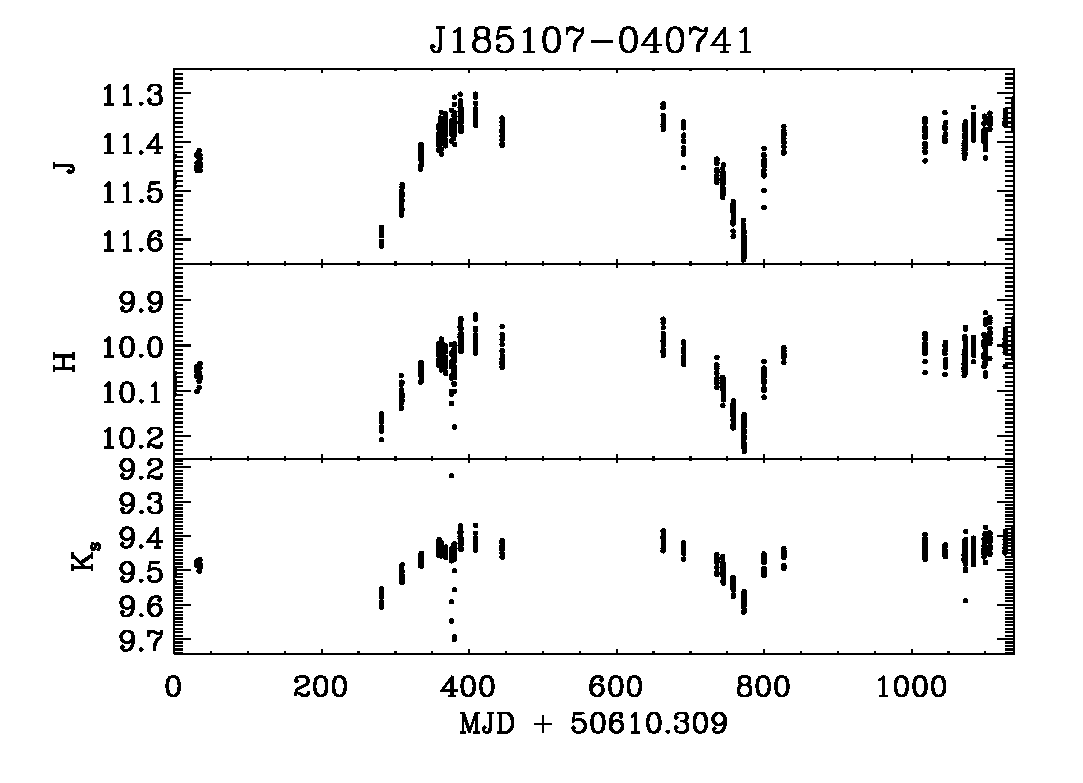
\includegraphics[width=2.0in]{plots/ll_22}\\
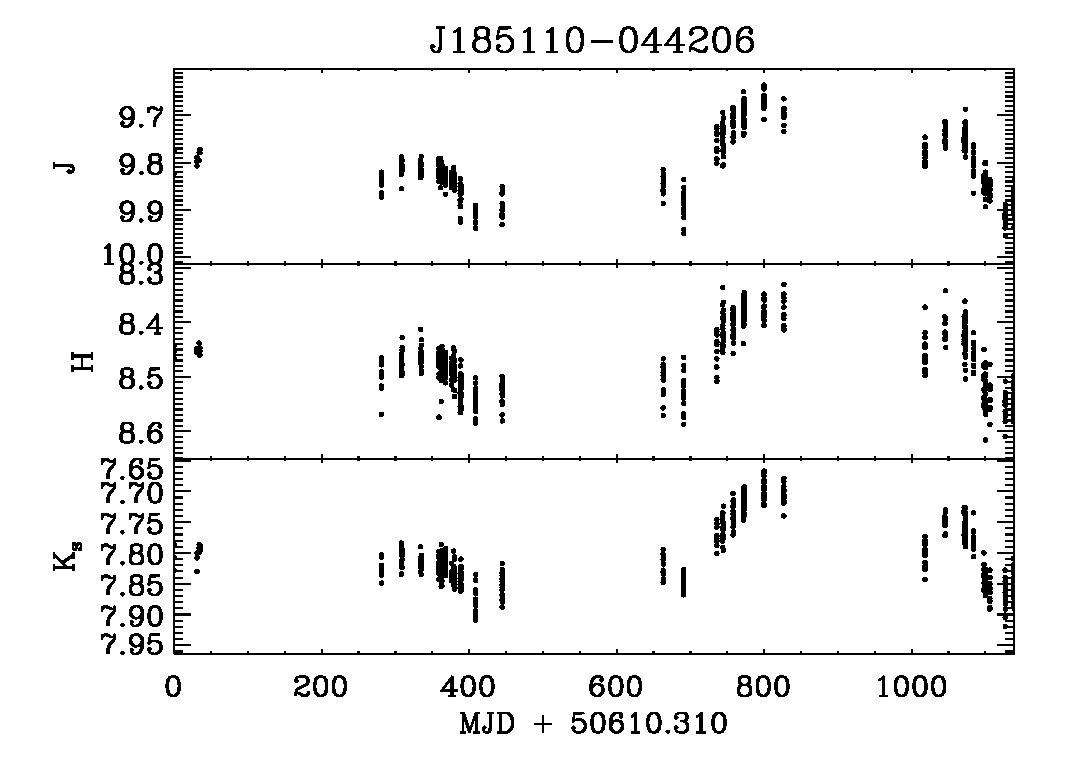
\includegraphics[width=2.0in]{plots/ll_23}
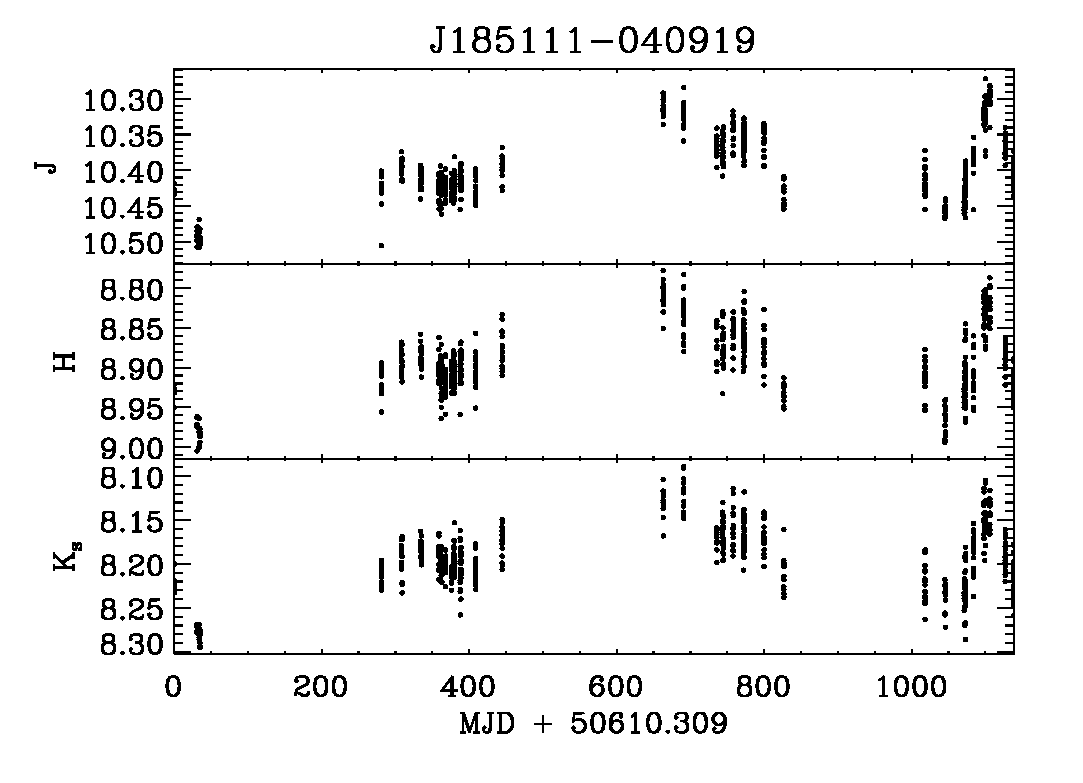
\includegraphics[width=2.0in]{plots/ll_24}
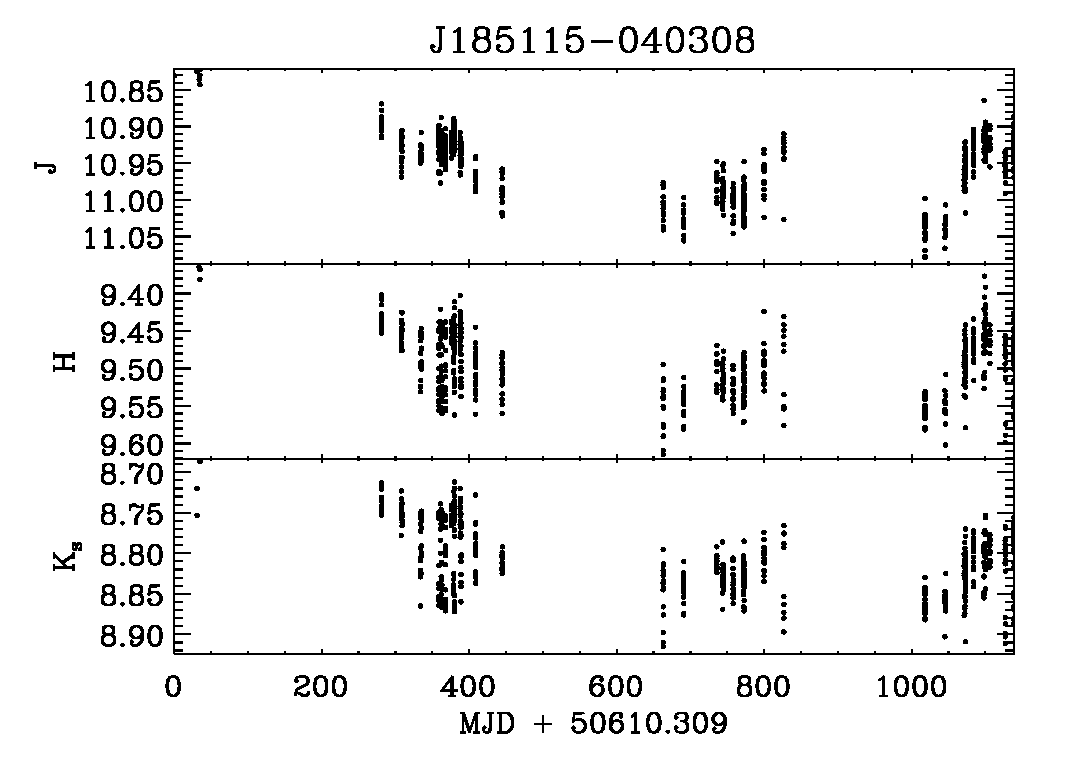
\includegraphics[width=2.0in]{plots/ll_25}\\
\includegraphics[width=2.0in]{plots/ll_26}
\includegraphics[width=2.0in]{plots/ll_30}
\includegraphics[width=2.0in]{plots/ll_32}\\
\includegraphics[width=2.0in]{plots/ll_36}
\includegraphics[width=2.0in]{plots/ll_40}
\includegraphics[width=2.0in]{plots/ll_41}
\caption{some long quasi-periodic variable objects. a couple look like DY Per's maybe? Nothing quite like RCB}
\label{ll}
\end{figure*}




%%%%%%%%%%%%%%%%%%%%%%%%%
%\section{Transient Objects}
% 
% have not been able to recover anything i believe...



%%%%%%%%%%%%%%%%%%%%%%%%%
\section{Variability Characteristics}

plots about ``color'' of variability, and overall trends

%%%%%%%%%%%%%%%%%%%%%%%%%%%%%
\section{Conclusions}



%%%%%%%%%%%%%%%%%%%%%%%%%
\acknowledgements
The authors acknowledge support from NASA ADP grant NNX09AC77G.

This publication makes use of data products from the Two Micron All Sky Survey, which is a joint project of the University of Massachusetts and the Infrared Processing and Analysis Center/California Institute of Technology, funded by the National Aeronautics and Space Administration and the National Science Foundation.

\bibliography{/Users/james/research/references}
\end{document}




